\chapter{Background}
\label{chap:background}

%What the chapter will say 
The findings acquired by this research study are based on theoretical models and principles of natural language processing, semantic web and game design. Having a clear understanding of the different components that compose the named entity disambiguation framework, conceptualizing the term "context" in relation to entity resolution and word sense disambiguation (\ac{wsd}) in general are the elements that this chapter will aim to clarify for the reader. Additionally, since the main contribution of this work is mainly focused on the gemification of non-game related tasks, and since the \ac{ned} framework provides the foundation on top of which game design principles will be applied, detailed insights on game design models and theories will be introduced in this chapter as well.   

%Body of chapter
\section{Linked Open Data (LOD) and the Web of Data concept}
Disambiguation of named entities by linking them with a knowledge base has many benefits that contribute in bringing the idea of Semantic Web of Data and the Linked Open Data principles closer to realization. Berners-Lee et al. \cite{lod_sofar} define \ac{lod} as follows: 

\begin{quote}
 "Linked Data is simply about using the Web to created typed links between data from different sources. It refers to data published on the Web in such a way that it is machine-readable, its meaning is explicitly defined, it is linked to other external data sets and can in turn be linked to and from other data sets.".\cite{lod_sofar}
\end{quote}

Furthermore, Tim Berners-Lee also argues that "\textit{The first step to semantic web is putting data on the web in a form that is understandable by machines or converting it to that form}" \cite{lod_sofar}. This is an important concept to shift our focus to, because it provides the means of publishing data on the web in such a way that all data published in the \ac{lod} will become part of a single global data space. The concept of Semantic Web should not be understood in alignment with the old and traditional "web of pages" where the main concern is putting data on the web. Semantic Web is about making links which should encourage exploration of the semantically connected web of data not only by humans but also by machines. Since the current WEB consists of large amount of unstructured information, based on the principles of \ac{lod} and Web of Data, it is necessary to convert this information to the desired form so that the goal of having a Semantic Web of Data is finally reached. "\textit{While semantic web, or web of data, is the goal for the end-result of this process, Linked Open Data provides the means to reach that goal}" \cite{lod_sofar}.

Our work contributes to the idea of semantic web and \ac{lod} principles in a way that it provides an effective and efficient way of semantically enriching unstructured web documents by disambiguation and linking the identified named entities with a \ac{kb} that is part of the \ac{lod} cloud (such as DBpedia) \cite{dbpedia}. Bauer et al. \cite{23} called Dbpedia "the semantic sister" of the most popular online encyclopedia in the world: Wikipedia, which makes Dbpedia one of the largest cross-domain knowledge bases extracted from the English edition of Wikipedia  \cite{23}. During the time of writing, Dbpedia is said to be the nucleus of the \ac{lod} cloud. It is one of the few \ac{kb} that has most in-links and out-links to other \ac{kb} published on the \ac{lod} cloud \cite{dbpedia, 23}. The so-called LOD-Cloud, covers more than an estimated 50 billion facts from many different domains like geography, multimedia, biology, politics, academia, energy and the like. Datasets published in the cloud are described with a unique language called "Resource Description Framework" or \ac{rdf} for short. It is a widely adopted standard for describing metadata as well as providing the means of structuring and linking data that describe things in the real world \cite{lod_sofar}. Figure \ref{fig:lod_diagram} represents the \ac{lod} Diagram as of 2017 and is constantly updated and maintained by the Linked Open Data initiative community \cite{lod-diagram}.

\begin{figure}[]
  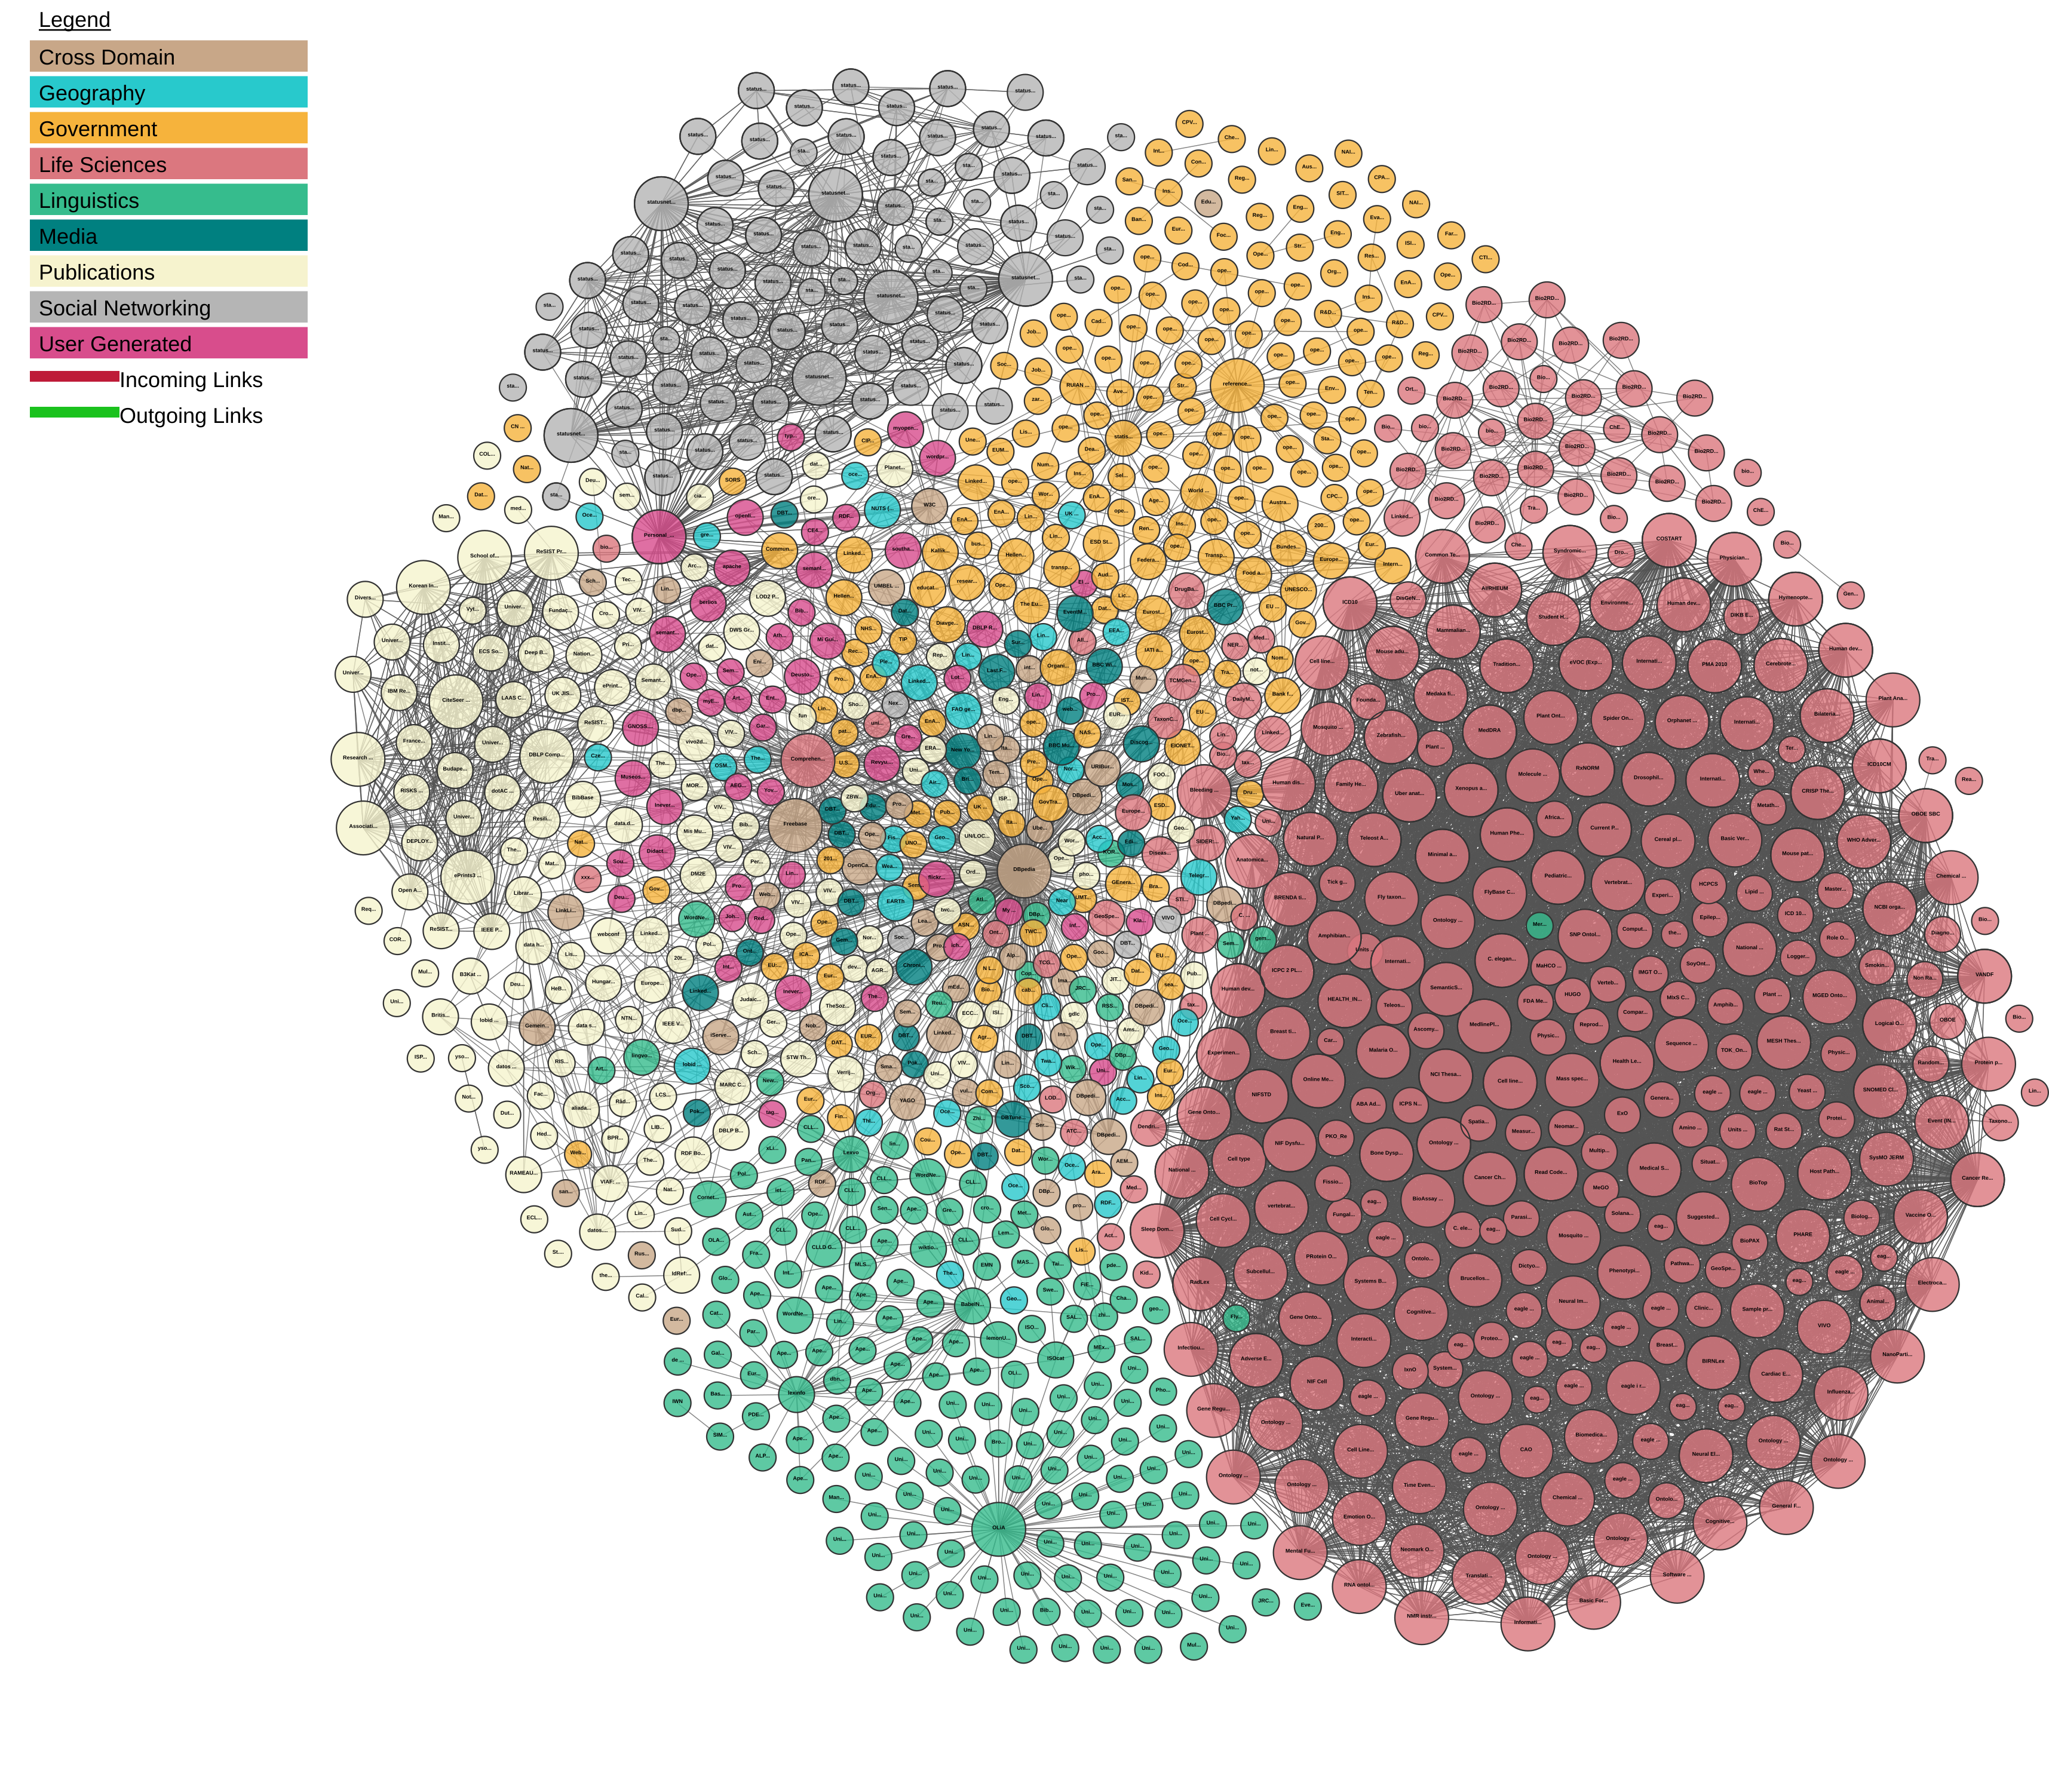
\includegraphics[width=\linewidth]{figures/lod.png}
  \caption{Linked Open Data cloud diagram 2017 \cite{lod-diagram}}
  \label{fig:lod_diagram}
\end{figure}

% - Named Entity Disambiguation 
\section{Named Entity Disambiguation (\ac{ned})}
The Named Entity Disambiguation term refers to the process of identifying potential entity mentions in textual data and linking them with the corresponding candidate from a \ac{kb} such as Dbpedia in our case. The disambiguation part from the complete term refers to selecting an entity candidate which accurately represents the named entities' meaning and sense based on the surrounding context. The so called concept of "Wikification" as explained by Trani et al. \cite{2} is a similar approach to \ac{ned} except that in their case the link associated with the entity mention corresponds to a Wikipedia page instead of an actual \ac{kb} link. 

Furthermore, \ac{ned} can also be explained by analyzing another similar NLP problem, that is, \ac{wsd} which stands for Word Sense Disambiguation. \cite{wsd} represents the task of determining the correct meaning (sense) of a word in a given context \cite{27}. \ac{wsd} is similar to entity linking/disambiguation\footnote{Please note that linking and disambiguation will be used interchangeably throughout the text, but will refer to the same conceptual idea of resolving an entity by first disambiguating it and then linking it to the knowledge base} in the sense that both problems refer to finding the correct reference of the spotted mention in an unstructured text document \cite{27}.

Defining the correct sense of a word or entity mention means knowing how to formulate the surrounding context which gives critical information to either the human or machine annotator for making an informed decision. The aforementioned process is considered as an AI-complete problem for machines, which in analogy to \ac{np}-completeness in complexity theory is a problem whose difficulty is equivalent to solving central problems of Artificial Intelligence (\ac{ai} \cite{30}. When attacking these problems in an automatic fashion using \ac{ai} algorithms, prior knowledge is required beforehand. According to Navigli \cite{30}, given a set of words, the procedure followed by a \ac{wsd} system starts by applying techniques which make use of one or more sources of knowledge to associate the most accurate senses with words in surrounding context. In analogy, \ac{ned} and \ac{wsd} can be seen as classification tasks where the candidate words or senses are the actual classes and usually an automatic classification algorithm is applied to assign a class to each named entity or word occurrence. The association should come as a result of making a decision that is based on evidence from the surrounding context and from potential external knowledge sources such as dictionaries \cite{30}. Although the approach investigated in our research study relies on manual human annotation, improving the automatic supervised classification techniques is the ultimate goal provided with enough training data.

Automatic approaches on the other hand can be classified in three different classes: 
\begin{itemize}
    \item Unsupervised,
    \item Semi-Supervised, and
    \item Supervised
\end{itemize}

Among these three categories, supervised approaches have proven to perform best in terms of accuracy and quality of annotations \cite{29}. Unsupervised approaches usually rely on unlabeled corpora, and do not utilize manually sense-tagged data to provide a sense choice for a word in context \cite{30}. Semi-supervised approaches, just like the name implies, also rely on unlabeled corpora but in addition to that, they use various classifiers which are trained on a smaller set of trained samples. 

In contrast to the previous approaches, supervised methods use machine learning techniques to learn classifiers from labeled training sets. Furthermore, feature sets such as Part-of-Speech (POS) of neighboring words, local collocations\footnote{Collocations are also known as bigrams. Bigrams represent a meaningful combination of two words}, syntactic patterns and other global features are used as strong classification features for the supervised methods \cite{27}. The fact that the later approach leads in terms of accuracy and performance does make it a favorable choice to use for discovering different solutions to NLP problems similar to \ac{ned} and \ac{wsd}. However, due to the data scarcity problem, relying on large-amount of training data for different domains, tasks and languages cannot be seen as a realistic assumption and therefore significant manual effort is required \cite{30}. According to Sanderson \cite{sanderson1994}, improvements in the performance of information retrieval systems would be observed only if problems such as \ac{ned} and \ac{wsd} would perform at a level of at least 90\% accuracy \cite{sanderson1994,30}. The only possible way of achieving high levels of performance on these kind of tasks is by training supervised algorithms with large amounts of training data. Investigating on techniques and methodologies that would assure the generation of large-scale training data while keeping costs at minimal levels and still maintaining quality is the focus of the upcoming chapters. Before proceeding to the next section, understanding what the term "context" refers to in our particular problem scope is the topic of the next subsection.


% - Defining Context 
\section{Defining Context}
\label{background:defininf_context}
Extracting information about the surrounding context of a word, an entity or even the context of the document as a whole (topic context) is one of the most important and yet most difficult tasks to achieve in \ac{nlp}. The surface form "Texas", according to Wikipedia, can refer to no more than twenty different named entities that can potentially describe the surface form based on the context it occurs. It may refer to the University of Texas, a Texas British Pop-Band, the US State of Texas or a novel named "Texas" written by Jams Michner \cite{24}. 

Context has the power of being virtually anything, and it can be seen as a container in which the phenomenon resides \cite{25}. It represents the parts of a discourse that surround a word or passage and can clarify the meaning or the interrelated conditions in which something exists or occurs \cite{22}. Bontas and Paslaru \cite{22} argue that contexts does not represent actual situations but it represents the perspective of an agent of the situation, since context is considered to be a partial approximation of a complete state of the world given a time point \cite{22,25}. Many studies see contextual information as a path that leads supervised algorithm or human annotator to make a clear decision on the disambiguation process of ambiguous surface forms (words). 

Furthermore, besides eliminating ambiguities, context may be used for completing the missing information in natural language utterances \cite{22}. The level of impact that context has in the performance of \ac{nlp} tasks, has taken the attention of many researchers who have been trying to formulate or define the context for many years \cite{35,37,28,29,26,38}. However, context processing largely depends on the application domain, and the procedures used to formulate it are way too specific to be used in a generic scope. Therefore, Bontas and Paslaru \cite{22} state that no clear and common methodology exists (yet) for the development of context-aware applications irrespective of the domain they belong to.   

Some of the most common used features for disambiguating the sense of an ambiguous word and also defining the surrounding context of a word include: surround words and their Part-Of-Speech (POS) tags, topic keywords, content bigrams and various syntactic properties \cite{36}. Topic keywords are considered as topical features that represent the general context of a document in which the ambiguous word resides. Unlike local features, topical features define the general topic of the document and represent a more generic context \cite{30}. On the other hand, local feature such as bi-grams and surround words are important to pin down more specific contextual information. Bigrams are ordered pairs of words that are judged statistically significant by a measure of association. They often provide very specific unambiguous clues regarding the content of a context \cite{26}. Navigli \cite{30} states that deciding on the appropriate size of context (the number of bigrams, surround words, topic keywords etc) is an important factor in the development of \ac{nlp} tasks such as \ac{ned} and \ac{wsd}. Inappropriate formulation of the context size is known to negatively affect the disambiguation performance of these tasks \cite{30}. 


\section{Game With A Purpose (GWAP)}
\label{thb:gamedesign}
%Why is gamification applied in our work
\if The advancement of technology has brought us many innovations and systems which contribute to facilitating everyday life and automating boring human workforce. However, the level of advancement has yet to reach the point where the human expertise is not required. Until then, many researchers are trying to explore ways in which particular boring tasks which are usually carried out by humans can become more interesting and exciting to do. \fi Gamification represents the idea of using game design principles for transforming a system which was originally not created as a fun activity into an engaging and interactive game with a purpose \cite{vonahn, 47}. In this study we elaborate on the potential of applying game design principles into the task of named entity disambiguation in order to achieve large-scale annotation data that can be used either as training data for supervised NLP algorithms or as a tool for enriching web documents with semantic meta-data.

%What is gamification - definitions
The proposed gamification approach of this research study and the field in which this technique is being applied, in literature is referred to as Games With A Purpose (\ac{gwap}) \cite{vonahn}.\ac{gwap} is one of the many approaches of gamification. The concept of gamification, as seen by researchers, involves applying elements of \textit{gamefulness, gameful interaction and gameful design} with a specific intention in mind. According to Seaborn et al. \cite{47}, \textit{gamefulness} refers to the lived experience, \textit{gameful interaction} refers to the object, tools and contexts that bring the feeling of gamefulness while \textit{gameful design} refers to the practice of creating a gameful experience. On the other hand, the aim of \ac{gwap} is to entertain players while they complete tasks that the system does not know, for most of the part, the correct answer. Usually, a well design \ac{gwap} harvests the knowledge of their players and acquires the solution to the underlying problems as a byproduct of players playing and interacting with the game \cite{vonahn}. Providing appropriate feedback at appropriate times during the gameplay for the players to feel engaged while using their knowledge and experience to solve \ac{nlp} problems presents a major challenge. Understanding the motivation of players in this scenario is key to the success of a \ac{gwap} \cite{43}.

%Why do we base our gamifying process on theoritical models 
Being able to guarantee, to some extent, that players will be engaged and motivated to play while interacting with the game, certain psychological needs have to be fulfilled so that players have the feeling of being immersively away from the real world and fully concentrated on the game. The answer to this question lies on theoretical cognitive theories such as the widely used Self-Determination Theory (\ac{sdt}) and its respective sub-theories \cite{std_and_games}. The process of designing the game for this particular research problem has been completely based on theoretical foundations and psychological theories for motivation (i.e. \ac{sdt}) in order to reach a state where players experience the feelings of being entertained. 

%What is SDT and CET, Intrinsic, extrinsic motivators and competance 
\ac{sdt}, is a macro theory of human motivation that is essentially concerned with the potential for social contexts to provide satisfying experience. In \ac{sdt}, the importance of competence (i.e. outcome control), autonomy (i.e. agency) and relatedness (i.e. connecting with others) are emphasized as the main factors to intrinsic motivation. Intrinsic motivation denotes the pursuit of an action because it is inherently enjoyable or interesting. In contrast, extrinsic motivation is defined as doing something due to a separable outcome, such as pressure or "extrinsic rewards" in the form of payment incentives or verbal feedback (ex. praise). Competence on the other hand, signifies the perceived extent of ones own actions as a cause of desired consequences and, as a psychological factor, is increased when the corresponding action is met with direct and positive feedback. It must be noted here that feelings of competence will not increase intrinsic motivation unless accompanied with a sense of autonomy. To affect feelings of autonomy, people must experience their actions and behaviour as self-determined rather than controlled by the system or an outside source. In support towards this concept, Cognitive Evaluation Theory (\ac{cet}), a sub-theory of \ac{sdt}, suggests that activities/actions foster greater intrinsic motivation when they provide goal-oriented tasks and an effort-full challenge. \cite{43, 49,std_and_games}

%Conclude chapter - what the chapter said, introduce the upcoming chapter
Understanding the theoretical foundations and ideas explained in this chapter is crucial to understanding and reasoning the contributions provided by this research study. In the next chapter, the implemented named entity disambiguation framework will be explored in great detail by first introducing the reader with state-of-the-art in the respective field and proceeding with technical and conceptual analysis of the different models and elements that build up the system.  